% ============================================================
%  PolyCongRÉ 2026 — Oral Presentation (7 min)
%  GAPF: Graph-Attentive Policy Fusion for WSN Routing
% ============================================================
\documentclass[aspectratio=169, 11pt]{beamer}

% ====================
% Packages
% ====================
\usepackage[T1]{fontenc}
\usepackage[utf8]{inputenc}
\usepackage{lmodern}
\usepackage{graphicx}
\usepackage{booktabs}
\usepackage{array}
\usepackage{amsmath,amssymb}
\usepackage{tikz}
\usetikzlibrary{positioning, arrows.meta, shapes.geometric, fit, decorations.pathreplacing, calc}
\usepackage{multirow}
\usepackage{xcolor}
\usepackage{caption}
\usepackage{appendixnumberbeamer}

% ====================
% Theme & Colors (Polytechnique Montréal inspired)
% ====================
\usetheme{Madrid}
\usecolortheme{default}

% Poly colors
\definecolor{polyblue}{RGB}{0, 70, 130}
\definecolor{polylightblue}{RGB}{0, 159, 223}
\definecolor{polygray}{RGB}{100, 100, 100}
\definecolor{polyred}{RGB}{200, 50, 50}
\definecolor{polygreen}{RGB}{0, 128, 80}
\definecolor{polyorange}{RGB}{230, 140, 20}

\setbeamercolor{structure}{fg=polyblue}
\setbeamercolor{palette primary}{bg=polyblue, fg=white}
\setbeamercolor{palette secondary}{bg=polylightblue, fg=white}
\setbeamercolor{palette tertiary}{bg=polyblue!80!black, fg=white}
\setbeamercolor{frametitle}{bg=polyblue, fg=white}
\setbeamercolor{title}{fg=white, bg=polyblue}
\setbeamercolor{block title}{bg=polyblue!15, fg=polyblue}
\setbeamercolor{block body}{bg=polyblue!5}
\setbeamercolor{block title alerted}{bg=polyred!15, fg=polyred}
\setbeamercolor{block body alerted}{bg=polyred!5}
\setbeamercolor{block title example}{bg=polygreen!15, fg=polygreen!80!black}
\setbeamercolor{block body example}{bg=polygreen!5}
\setbeamercolor{item}{fg=polyblue}
\setbeamercolor{itemize item}{fg=polyblue}
\setbeamercolor{itemize subitem}{fg=polylightblue}
\setbeamercolor{enumerate item}{fg=polyblue}

\setbeamertemplate{navigation symbols}{}
\setbeamertemplate{footline}{%
  \leavevmode%
  \hbox{%
    \begin{beamercolorbox}[wd=.4\paperwidth,ht=2.5ex,dp=1.125ex,leftskip=.3cm]{author in head/foot}%
      \usebeamerfont{author in head/foot}\insertshortauthor
    \end{beamercolorbox}%
    \begin{beamercolorbox}[wd=.35\paperwidth,ht=2.5ex,dp=1.125ex,center]{title in head/foot}%
      \usebeamerfont{title in head/foot}\textit{PolyCongR\'{E} 2026}
    \end{beamercolorbox}%
    \begin{beamercolorbox}[wd=.25\paperwidth,ht=2.5ex,dp=1.125ex,rightskip=.3cm plus1fil]{date in head/foot}%
      \hfill\insertframenumber\,/\,\inserttotalframenumber
    \end{beamercolorbox}}%
  \vskip0pt%
}

% ====================
% Metadata
% ====================
\title[GAPF for WSN Routing]{Energy-Efficient and Near Real-Time Routing\\for Disaster Monitoring in Wireless Sensor Networks}
\subtitle{Graph-Attentive Policy Fusion (GAPF)}
\author[G.\,P.\,Djimefo Kapen]{%
  \textbf{Georges Parfait Djimefo Kapen}\\[4pt]
  {\small Director: \textbf{Pr.\,Ranwa Al Mallah}}\\
  {\small Co-director: \textbf{Pr.\,Samuel Pierre}, Senior Member, IEEE}}
\institute[Polytechnique Montréal]{%
  Mobile Computing and Networking Research Laboratory (LARIM)\\
  Dept.\ of Computer and Software Engineering\\
  Polytechnique Montr\'{e}al}
\date{PolyCongR\`{E}s 2026}

% Logos
\titlegraphic{%
  \vspace{-0.5cm}%
  
\includegraphics[height=1.2cm]{./logos/LogoPoly.png}%
  \hspace{1.5cm}%
  
\includegraphics[height=1.2cm]{./logos/LogoLarim.png}%
}

\logo{%
  
\includegraphics[height=0.6cm]{./logos/LogoPoly.png}%
  \hspace{0.3cm}%
  
\includegraphics[height=0.6cm]{./logos/LogoLarim.png}%
  \hspace{0.3cm}%
}


% ====================
% Document
% ====================
\begin{document}

% ────────────────────────────────────────────────────────────
% SLIDE 1 — Title  (~30 s)
% ────────────────────────────────────────────────────────────
\begin{frame}[plain]
  \titlepage
\end{frame}

% ────────────────────────────────────────────────────────────
% SLIDE 2 — Outline  (~15 s)
% ────────────────────────────────────────────────────────────
\begin{frame}{Outline}
  \tableofcontents
\end{frame}

% ============================================================
\section{Context \& Motivation}
% ============================================================

% ────────────────────────────────────────────────────────────
% SLIDE 3 — Why Disaster Monitoring Matters  (~50 s)
% ────────────────────────────────────────────────────────────
\begin{frame}{Why Disaster Monitoring Matters}

\begin{columns}[T]
\begin{column}{0.55\textwidth}

  \begin{alertblock}{A Real-World Crisis}
    \vspace{-2pt}
    In \textbf{2023}: \textbf{398} natural disasters, \textbf{95\,000} deaths, \textbf{\$380\,B} in losses
    \vspace{-2pt}
    \par{\scriptsize\textit{Source: EEA, Statista 2023}}
  \end{alertblock}

  \smallskip
  \textbf{Wireless Sensor Networks (WSNs)} are essential tools:
  \begin{itemize}\setlength{\itemsep}{1pt}
    \item Self-configuring, infrastructure-independent
    \item Accurate data with minimal human intervention
    \item Resilient when infrastructure is destroyed
  \end{itemize}

\end{column}
\begin{column}{0.42\textwidth}
  \centering
  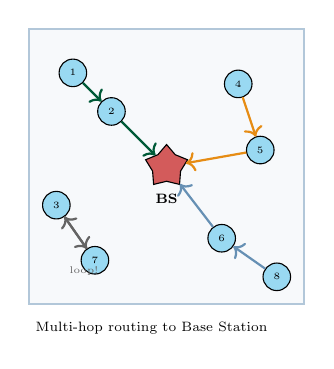
\begin{tikzpicture}[scale=0.7, every node/.style={scale=0.7}]
    % Field
    \draw[thick, polyblue!30, fill=polyblue!3] (0,0) rectangle (5,5);
    % BS
    \node[draw, fill=polyred!80, star, star points=5, minimum size=8mm, inner sep=0pt] (bs) at (2.5,2.5) {};
    \node[below=2pt of bs, font=\scriptsize\bfseries] {BS};
    % Sensors
    \foreach \x/\y/\n in {0.8/4.2/1, 1.5/3.5/2, 0.5/1.8/3, 3.8/4.0/4, 4.2/2.8/5, 3.5/1.2/6, 1.2/0.8/7, 4.5/0.5/8}{
      \node[draw, circle, fill=polylightblue!40, minimum size=5mm, inner sep=0pt, font=\tiny] (s\n) at (\x,\y) {\n};
    }
    % Arrows (multi-hop routes)
    \draw[->, thick, polygreen!70!black] (s1) -- (s2);
    \draw[->, thick, polygreen!70!black] (s2) -- (bs);
    \draw[->, thick, polyorange] (s4) -- (s5);
    \draw[->, thick, polyorange] (s5) -- (bs);
    \draw[->, thick, polyblue!60] (s8) -- (s6);
    \draw[->, thick, polyblue!60] (s6) -- (bs);
    \draw[->, thick, polygray] (s3) -- (s7);
    \draw[->, thick, polygray] (s7) -- (s3);
    \node[below, font=\tiny, text=polygray] at (1.0,0.8) {loop!};
    % Legend
    \node[font=\scriptsize, anchor=north west] at (0,-0.2) {Multi-hop routing to Base Station};
  \end{tikzpicture}
\end{column}
\end{columns}

\vspace{2pt}
\centering
\colorbox{polyblue!10}{\parbox{0.9\textwidth}{\centering
  \textbf{Core tension:} Deliver all data reliably \textit{vs.}\ Preserve limited battery energy
}}

\end{frame}

% ────────────────────────────────────────────────────────────
% SLIDE 4 — Limitations of Existing Approaches  (~50 s)
% ────────────────────────────────────────────────────────────
\begin{frame}{Limitations of Current Approaches}

\begin{columns}[T]
\begin{column}{0.48\textwidth}

  \begin{block}{Metaheuristic Methods {\small(PSO, Firefly, GWO\ldots)}}
    \begin{itemize}\setlength{\itemsep}{1pt}
      \item[\textcolor{polyred}{\textbullet}] Assume \textbf{static} sensor positions
      \item[\textcolor{polyred}{\textbullet}] No adaptation to topology changes
      \item[\textcolor{polyred}{\textbullet}] PDR \textbf{collapses $<$10\%} at scale
    \end{itemize}
  \end{block}

  \smallskip
  \begin{block}{Single-Agent RL (Q-learning)}
    \begin{itemize}\setlength{\itemsep}{1pt}
      \item[\textcolor{polyred}{\textbullet}] Reward = simple \textbf{weighted sum}
      \item[\textcolor{polyred}{\textbullet}] Cannot capture multi-objective complexity
    \end{itemize}
  \end{block}

\end{column}
\begin{column}{0.48\textwidth}

  \begin{block}{Multi-Agent RL (QMIX, QTRAN)}
    \begin{itemize}\setlength{\itemsep}{1pt}
      \item[\textcolor{polyorange}{\textbullet}] QMIX: limited by \textbf{monotonicity} constraint
      \item[\textcolor{polyorange}{\textbullet}] QTRAN: better theory, \textbf{harder to train}
      \item[\textcolor{polyred}{\textbullet}] Both \textbf{ignore network topology}
      \item[\textcolor{polyred}{\textbullet}] \textbf{Memory explosion}: up to \textbf{13.8\,GB}
    \end{itemize}
  \end{block}

  \smallskip
  \begin{exampleblock}{Our Goal}
    Design a \textbf{lightweight, topology-aware} meta-controller that selects the best routing expert while satisfying \textbf{energy, latency, and memory} constraints.
  \end{exampleblock}

\end{column}
\end{columns}

\end{frame}


% ============================================================
\section{Proposed Framework: GAPF}
% ============================================================

% ────────────────────────────────────────────────────────────
% SLIDE 5 — GAPF Overview  (~1 min)
% ────────────────────────────────────────────────────────────
\begin{frame}{GAPF: Graph-Attentive Policy Fusion --- Overview}

\begin{columns}[T]
\begin{column}{0.55\textwidth}

  \textbf{Three key contributions:}
  \begin{enumerate}\setlength{\itemsep}{2pt}
    \item \textbf{GAPF Meta-Controller}\\
      {\small GCN encodes WSN topology $\to$ CAS selects best expert per episode. Only \colorbox{polyblue!10}{\textbf{1\,473 params}}.}

    \item \textbf{Monotonic Attention Reward}\\
      {\small Learned attention scalarizes 4 objectives with \textbf{monotonicity guarantee}. Tuned by \textbf{Evolution Strategies}.}

    \item \textbf{Realistic Gym Environment}\\
      {\small Dynamic sensor mobility, energy-aware multi-hop, custom OpenAI Gym.}
  \end{enumerate}

\end{column}
\begin{column}{0.42\textwidth}
  \centering
  \vspace{-8pt}
  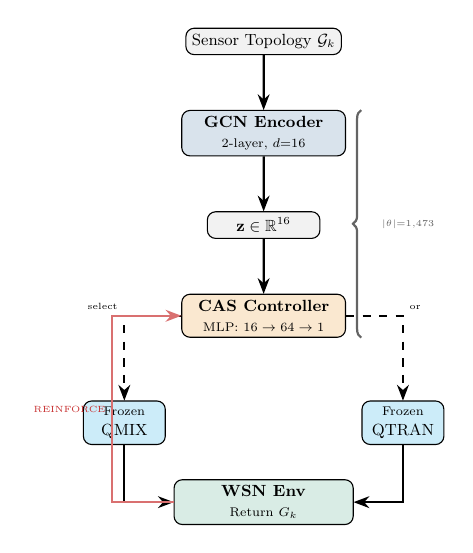
\begin{tikzpicture}[
      scale=0.65, every node/.style={scale=0.65},
      node distance=0.7cm,
      box/.style={draw, rounded corners=3pt, minimum height=0.7cm, minimum width=3.2cm, align=center, font=\small},
      data/.style={draw, rounded corners=3pt, minimum height=0.5cm, minimum width=2.2cm, align=center, fill=gray!10, font=\small},
      arrow/.style={-{Stealth[length=2mm]}, thick},
      dasharrow/.style={-{Stealth[length=2mm]}, thick, dashed},
    ]
    \node[data] (topo) {Sensor Topology $\mathcal{G}_k$};
    \node[box, below=of topo, fill=polyblue!15] (gcn) {\textbf{GCN Encoder}\\{\scriptsize 2-layer, $d{=}16$}};
    \node[data, below=of gcn] (embed) {$\mathbf{z} \in \mathbb{R}^{16}$};
    \node[box, below=of embed, fill=polyorange!20] (cas) {\textbf{CAS Controller}\\{\scriptsize MLP: $16 \to 64 \to 1$}};
    \node[box, below left=0.8cm and 0.2cm of cas, fill=polylightblue!20, minimum width=1.6cm] (qmix) {\scriptsize Frozen\\QMIX};
    \node[box, below right=0.8cm and 0.2cm of cas, fill=polylightblue!20, minimum width=1.6cm] (qtran) {\scriptsize Frozen\\QTRAN};
    \node[box, below=1.8cm of cas, fill=polygreen!15, minimum width=3.5cm] (env) {\textbf{WSN Env}\\{\scriptsize Return $G_k$}};
    % Arrows
    \draw[arrow] (topo) -- (gcn);
    \draw[arrow] (gcn) -- (embed);
    \draw[arrow] (embed) -- (cas);
    \draw[dasharrow] (cas) -| node[above left, font=\tiny]{select} (qmix);
    \draw[dasharrow] (cas) -| node[above right, font=\tiny]{or} (qtran);
    \draw[arrow] (qmix) |- (env);
    \draw[arrow] (qtran) |- (env);
    \draw[arrow, polyred!70, thick] (env.west) -- ++(-1.2,0) |- (cas.west)
      node[pos=0.25, left, font=\tiny, text=polyred, align=right] {REINFORCE};
    % Brace
    \draw[decorate, decoration={brace, amplitude=3pt, mirror}, thick, polygray]
      let \p1=(gcn.north east), \p2=(cas.south east) in
      (\x1+0.3cm, \y1) -- (\x1+0.3cm, \y2)
      node[midway, right=5pt, font=\tiny, text=polygray, align=left] {$|\theta|{=}1{,}473$};
  \end{tikzpicture}
\end{column}
\end{columns}

\end{frame}

% ────────────────────────────────────────────────────────────
% SLIDE 6 — Reward Design  (~50 s)
% ────────────────────────────────────────────────────────────
\begin{frame}{Bi-Level Reward Architecture}
\vspace{-8pt}
\begin{columns}[T]
\begin{column}{0.50\textwidth}

  \textbf{Inner level:} 4-dim reward vector per hop
  \vspace{-6pt}
  \[
    \mathbf{r}_i^{(t)} = \bigl[\;\underbrace{r_1}_{\text{angle}},\;\underbrace{r_2}_{\text{energy}},\;\underbrace{r_3}_{\text{balance}},\;\underbrace{r_4}_{\text{load}}\;\bigr] \in [0,1]^4
  \]

  \vspace{-4pt}
  \textbf{Attention weighting} (learned, input-independent):
  \vspace{-6pt}
  \[
    \alpha_j = \frac{\exp(\mathbf{k}_j^\top \mathbf{q}/\sqrt{d})}{\sum_{l=1}^{4}\exp(\mathbf{k}_l^\top \mathbf{q}/\sqrt{d})}
  \]

  \vspace{-6pt}
  \textbf{Monotonic network} ($4 \!\to\! 16 \!\to\! 16 \!\to\! 1$):\;
  $\mathbf{W}_\ell \!\geq\! 0$ via softplus\\
  $\Rightarrow$ \textbf{Pareto-dominating action always gets higher reward}

\end{column}
\begin{column}{0.47\textwidth}

  \begin{block}{Outer level: Evolution Strategies}
    \vspace{-4pt}
    Meta-objective after each episode:
    \vspace{-6pt}
    {\small\[
      J = \underbrace{1 - \tfrac{\sum(E_0 - e_i^{\text{rem}})}{N \cdot E_0}}_{\text{energy eff.}} + \underbrace{1 - \tfrac{\sigma(\mathbf{e}_{\text{rem}})}{E_0/2}}_{\text{energy bal.}}
    \]}
    \vspace{-10pt}
    \begin{itemize}\setlength{\itemsep}{0pt}
      \item[$\to$] Decouples reward shaping from RL gradient
      \item[$\to$] Adapts weights to each topology
    \end{itemize}
  \end{block}

  \smallskip
  \begin{exampleblock}{Why is this novel?}
    \begin{itemize}\setlength{\itemsep}{0pt}
      \item No manual weight tuning
      \item Mathematically guaranteed monotonicity
      \item Generalizes across topologies
    \end{itemize}
  \end{exampleblock}

\end{column}
\end{columns}

\end{frame}


% ============================================================
\section{Experimental Results}
% ============================================================

% ────────────────────────────────────────────────────────────
% SLIDE 7 — Results: PDR & Energy  (~1 min)
% ────────────────────────────────────────────────────────────
\begin{frame}{Results: Packet Delivery \& Energy Efficiency}
  {\small 7 scenarios $\times$ 3 seeds $\times$ 1\,000 episodes = \textbf{21\,000 test episodes}}

\begin{columns}[T]
\begin{column}{0.48\textwidth}

  \begin{block}{Packet Delivery Ratio (PDR)}
  \centering
  \footnotesize
  \renewcommand{\arraystretch}{1.1}
  \begin{tabular}{cc|cc|>{\bfseries}c}
    \toprule
    $n$ & $R$ & QMIX & QTRAN & GAPF \\
    \midrule
    20  & 25 & .559 & .558 & \textbf{.753} \\
    30  & 25 & .568 & .567 & \textbf{.877} \\
    50  & 35 & .553 & .552 & \textbf{.990} \\
    70  & 35 & .545 & .545 & \textbf{.980} \\
    100 & 35 & .464 & .462 & \textbf{.980} \\
    100 & 50 & .669 & .684 & \textbf{.980} \\
    \bottomrule
  \end{tabular}

  \vspace{4pt}
  \textcolor{polygreen}{\textbf{+43\% to +111\%}} relative improvement
  \end{block}

\end{column}
\begin{column}{0.48\textwidth}

  \begin{block}{Energy Balance ($\sigma_E$, $\downarrow$ better)}
  \centering
  \footnotesize
  \renewcommand{\arraystretch}{1.1}
  \begin{tabular}{cc|cc|>{\bfseries}c}
    \toprule
    $n$ & $R$ & QMIX & QTRAN & GAPF \\
    \midrule
    20  & 25 & .0075 & .0075 & \textbf{.0043} \\
    30  & 25 & .0111 & .0112 & \textbf{.0035} \\
    50  & 35 & .0264 & .0265 & \textbf{.0039} \\
    70  & 35 & .0318 & .0319 & \textbf{.0049} \\
    100 & 35 & .0455 & .0457 & \textbf{.0061} \\
    100 & 50 & .0559 & .0559 & \textbf{.0061} \\
    \bottomrule
  \end{tabular}

  \vspace{4pt}
  \textcolor{polygreen}{\textbf{3--9$\times$}} better energy balance
  \end{block}

\end{column}
\end{columns}

\vspace{6pt}
\centering
\colorbox{polyblue!10}{\parbox{0.85\textwidth}{\centering
  QMIX $\approx$ QTRAN ($<$2\% gap): gain comes from \textbf{topology-aware fusion}, not from expert choice alone
}}

\end{frame}

% ────────────────────────────────────────────────────────────
% SLIDE 8 — Deployment Feasibility  (~50 s)
% ────────────────────────────────────────────────────────────
\begin{frame}{Deployment Feasibility: From Server to Sensor}
\vspace{-2pt}
\begin{columns}[T]
\begin{column}{0.50\textwidth}

  \begin{block}{Feasibility Compliance}
  \centering
  \footnotesize
  \renewcommand{\arraystretch}{1.15}
  \begin{tabular}{l|cc|c}
    \toprule
    \textbf{Metric} & \textbf{QMIX} & \textbf{QTRAN} & \textbf{GAPF} \\
    \midrule
    Peak RAM & \multicolumn{2}{c|}{3.2--13.8\,GB} & \textbf{684--951\,MB} \\
    Mem $<$1\,GB? & \textcolor{polyred}{\textbf{FAIL}} & \textcolor{polyred}{\textbf{FAIL}} & \textcolor{polygreen}{\textbf{PASS}} \\
    Latency $p_{95}$ & 0.27\,ms & 0.17\,ms & \textbf{0.03\,ms} \\
    \bottomrule
  \end{tabular}
  \end{block}

  \medskip
  \begin{exampleblock}{CTDE Paradigm}
    \begin{itemize}
      \item \textbf{Training:} heavy components on server
      \item \textbf{Deployment:} only lightweight GRU on each sensor
      \item Mixers, reward network, ES loop $\to$ \textbf{discarded}
    \end{itemize}
  \end{exampleblock}

\end{column}
\begin{column}{0.47\textwidth}

  \begin{block}{What Runs on the Sensor?}
  \centering
  \footnotesize
  \renewcommand{\arraystretch}{1.15}
  \begin{tabular}{lc}
    \toprule
    \textbf{Resource} & \textbf{Requirement} \\
    \midrule
    Flash (weights) & $\sim$100\,KB \\
    SRAM (runtime) & $\sim$2\,KB \\
    Compute/step & $\sim$29K MACs \\
    Inference time & $<$1\,ms \\
    \bottomrule
  \end{tabular}

  \vspace{6pt}
  \normalsize
  \textbf{Compatible with:}\\[2pt]
  {\small STM32L4 (1\,MB flash, 256\,KB SRAM)\\
  nRF52840 (1\,MB flash, 256\,KB RAM)}
  \end{block}

  \vspace{4pt}
  \centering
  \colorbox{polyorange!15}{\parbox{0.95\columnwidth}{\centering\small
    GAPF adds \textbf{zero overhead}\\on sensor nodes
  }}

\end{column}
\end{columns}

\end{frame}


% ============================================================
\section{Impact \& Conclusion}
% ============================================================

% ────────────────────────────────────────────────────────────
% SLIDE 9 — Real-World Impact  (~50 s)
% ────────────────────────────────────────────────────────────
\begin{frame}{Real-World Impact}

\begin{columns}[T]
\begin{column}{0.48\textwidth}

  \begin{block}{\textcolor{polyred}{$\heartsuit$} Life-Saving Responsiveness}
    \begin{itemize}\setlength{\itemsep}{1pt}
      \item $\geq$\textbf{98\% packet delivery} at all scales
      \item Every undelivered reading = \textbf{blind spot}
      \item Near real-time: $<$1\,ms per routing decision
    \end{itemize}
  \end{block}

  \smallskip
  \begin{block}{\textcolor{polygreen}{$\bigstar$} Green AI}
    \begin{itemize}\setlength{\itemsep}{1pt}
      \item \textbf{2--3.5$\times$} less energy $\Rightarrow$ longer lifetime
      \item Fewer batteries in disaster zones; less e-waste
      \item Only \textbf{1\,473 parameters} to train
    \end{itemize}
  \end{block}

\end{column}
\begin{column}{0.48\textwidth}

  \begin{block}{\textcolor{polyblue}{$\blacktriangleright$} Broader Applicability}
    \textit{``Lightweight policy fusion $>$ monolithic models''}
    \begin{itemize}\setlength{\itemsep}{1pt}
      \item Vehicular ad-hoc networks (VANETs)
      \item Drone swarm coordination
      \item Smart grid load balancing
    \end{itemize}
  \end{block}

  \smallskip
  \begin{alertblock}{Responsible AI}
    \begin{itemize}\setlength{\itemsep}{1pt}
      \item \textbf{Interpretable}: binary selection is auditable
      \item \textbf{Efficient}: minimal training compute
      \item \textbf{Deployable}: no GPU at inference
    \end{itemize}
  \end{alertblock}

\end{column}
\end{columns}

\end{frame}

% ────────────────────────────────────────────────────────────
% SLIDE 10 — Conclusion & Future Work  (~40 s)
% ────────────────────────────────────────────────────────────
\begin{frame}{Conclusion \& Future Work}
\vspace{-4pt}
\begin{block}{Summary of Key Results}
\centering
\footnotesize
\renewcommand{\arraystretch}{1.1}
\begin{tabular}{lc}
  \toprule
  \textbf{Achievement} & \textbf{Result} \\
  \midrule
  Packet Delivery Ratio & $\geq$\textbf{98\%} (20--100 sensors) \\
  PDR improvement vs.\ baselines & \textbf{+43\% to +111\%} \\
  Energy reduction & \textbf{2--3.5$\times$} less than QMIX/QTRAN \\
  Energy balance & \textbf{3--9$\times$} better \\
  Memory reduction & \textbf{13$\times$} less (951\,MB vs.\ 13.2\,GB) \\
  Trainable parameters & Only \textbf{1\,473} \\
  Feasibility constraints & \textcolor{polygreen}{\textbf{ALL PASSED}} \\
  \bottomrule
\end{tabular}
\end{block}

\vspace{-2pt}
\smallskip
\textbf{Future directions:}
\begin{enumerate}\setlength{\itemsep}{1pt}
  \item Hardware-in-the-loop on nRF52840 motes
  \item Cross-domain: flood, wildfire, earthquake monitoring
  \item Dynamic step-level expert fusion
  \item Multi-expert generalization ($>$2 experts)
\end{enumerate}

\end{frame}

% ────────────────────────────────────────────────────────────
% SLIDE 11 — Thank You / Questions
% ────────────────────────────────────────────────────────────
\begin{frame}[plain]

\vfill
\begin{center}

  {\Large\bfseries\textcolor{polyblue}{Thank You!}}

  \bigskip
  {\large Questions?}

  \bigskip\bigskip

  \textbf{Georges Parfait Djimefo Kapen}\\[4pt]
  {\small Director: Pr.\,Ranwa Al Mallah \quad|\quad Co-director: Pr.\,Samuel Pierre}\\[6pt]
  {\small\texttt{georges-parfait.djimefo-kapen@polymtl.ca}}

  \bigskip
  
\includegraphics[height=1.2cm]{./logos/LogoPoly.png}%
  \hspace{2cm}%
  
\includegraphics[height=1.2cm]{./logos/LogoLarim.png}

  \medskip
  {\footnotesize PolyCongR\`{E}s --- Congr\`es \'{e}tudiant de recherche en g\'{e}nie\\
  Polytechnique Montr\'{e}al, 2026}

\end{center}
\vfill

\end{frame}

\end{document}
